\documentclass{article}
\usepackage{amsmath}
\usepackage[fleqn]{mathtools}
\usepackage{amssymb}
\usepackage{amsthm}
\usepackage{enumitem}
\usepackage{float}
\usepackage[dvips,xetex]{graphicx}
\usepackage{caption}
\usepackage{subcaption}
\usepackage[linesnumbered,ruled]{algorithm2e}
\begin{document}
	\title{Multi-actor network repair problems}
	\author{Brian French}
	\maketitle
	\section{Status Tracker}
	\begin{itemize}
		\item Introduction -- started
		\item Literature Review - started
		\item Modeling - drafted
		\item Results/conclusions -started
		\item Resilience -- started
		\item Conclusions -- thought about
	\end{itemize}
	
	\section{Introduction and Motivation}
	Hurricanes are a growing concern in the operation of power grids in coastal areas. This is due partly to the increasing density of cities in coastal areas, but the impacts of climate change are causing both rising sea levels making flooding worse, but also more frequent and more severe hurricanes \cite{MannEA2006}. This phenomenon suggests that repair procedures and resilience planning will be of increased importance in the coming years.
	
	This thesis explores the gap in existing literature where previous efforts have not explicitly considered how multiple networks depended on each other, especially the post-disaster infrastructure recovery interactions between power grid and road networks. For example, to repair a damaged power grid element, the element must be accessible to the crew attempting to repair it. Moreover, the crew will take time to go from one element to the next to repair, affecting the power grid's performance during recovery. This implies that the road network (how damaged it is and how its recovery is planned) becomes part of the overall recovery efforts. During a hurricane, the road network will sustain substantial damage from flooding and debris on the road surface, which necessitates road grid repairs/clearance as well. To handle the issues of repairing power grids efficiently, both types of repairs (road network and power grid) should be considered jointly. Previous literature does not study this specific interaction as discussed in the section below.

	Understanding of repair efforts on power grids begins with understanding the basics of power grid topology. We divide the power grid into transmission and distribution networks. Transmission consists of generators, buses/substations, and high voltage connecting lines. Because this side of the grid has multiple sources and sinks, flow is not guaranteed to flow in a certain direction. The distribution side of a network begins at the bus/substation level and connects end users of power to the grid as a whole. Because power flows from the substation to the end user in a single source network, these networks are comparatively simpler to model. For the sake of this thesis, we restrict ourselves to just transmission level power grids as distribution grids are simpler at an electrical level as well as being geographically small enough that ignoring routing time costs doesn't stray from optimality very far.
	\section{Literature Review}
	\subsection{Hurricane Damage Modeling}
		When delving into the background literature, no discussion of modeling repair after a hurricane can happen before looking at the literature on damage to power grids from hurricanes. \cite{GuikemaEA2010} use a model based on negative binomial regression to estimate the number of downed power lines in combination with a classification tree handling flooding and wind speed over/under 100 miles per hour. \cite{ScherbEA2015} on the other hand takes an approach more rooted in scenario generation and tries to use the peak windspeed and proximity to the eye wall of a hurricane to construct a loss function for power lines. Both of these papers come to the similar conclusion that damage to 40-70\% of power lines due to wind and thrown debris is common in hurricanes.
		
		 \cite{WinklerEA2010} Provides the most thorough analysis of these 3 papers using real world topographies from various small regions of Texas and coming up with loss functions for both lines and substations. Worth noting in all three of these examples is that lines and substations sustain the most damage, but generators themselves are robust enough that a hurricane is unlikely to damage them. This means they can be ignored in the repair modeling later on. This validated the later modeling of how damage happens to a power grid in the wake of a hurricane.
	\subsection{Existing Power Grid Repair Modeling}
		Power grid repairs in the wake of hurricanes are not an unstudied area of research. \cite{NPSMasters} solves a scheduling problem of power grid repair in the wake of both hurricanes and terrorist attacks. While they don't consider impacts of roads, they do significant work with how to model a damaged power grid. Along similar lines, \cite{ArabEA2015} solve a similar problem under uncertainty by treating the state of each power line and generator as a random Bernoulli variable and solving the ensuing stochastic 
		optimization problem. 
		
		\cite{OuyangEA2014} Does a statistical analysis of the rate at which damage is recovered in the context of broader power grid resilience. While more descriptive than prescriptive, they do lay out that transmission grid repairs take priority alongside "critical facilities vital to public safety, health, and welfare".
		
		\cite{GolariEA2014} Takes a different approach to ensuring power demand satisfaction in the context of a damaged power network by approaching the problem in the lens of construction of sub-grids (termed "islands" in much of the electrical engineering literature) in order to keep demand satisfied in a post-disaster context.
	\subsection{Existing Road Grid Repair Modeling}
		\cite{PregnolatoEA2017} provides an overview of probability of road damage by location and intensity. They go on to provide a literature review and meta-analysis of existing papers in the subfield. They then go on to summarize a variety of versions of depth-disruption functions for roads based on local rain intensity. Alone this paper doesn't add significant amounts to modeling repair efforts, but it does provide insights into how flooding is addressed at the analysis level.
		
		Looking next at how previous papers have addressed modeling flooding and how to interact with it in a repair context, we start with \cite{DuqueEA2016}. This paper focuses on distribution of relief supplies, but in the context of the problem of supply distribution they consider repair of flooded or damaged roads. Though solve the problem with dynamic programming, it is from this paper where we take the idea of repair of roads by traversing them at additional cost.
		
		Also of note from the perspective of road repair is \cite{AksuEA2014}. Again not a paper focused focused on direct repair of networks for its own sake, but rather a paper focused on evacuation and accessibility to areas flooded by the a disaster. This provides additional insight and a different treatment of the problem using mixed integer programming rather than the dynamic programming of Duque et al. From this, we draw inspiration for treatment of the road grid
	
	\subsection{Resilience}
	

	\subsection{Scenario Generation}
	\section{Repair Problem}
	
	\subsection{Overview}
	To motivate the problem, we see from the literature a gap in looking at power grid repairs in a post-disaster context with consideration of the roads. The Federal Emergency Management Agency's 2017 post season after action report\cite{FEMA2017AAR}  and Hurricane Sandy after action report \cite{FEMASandyAAR} make note of the need of increased coordination between agencies for the sake of logistics as well as it having been a major short coming in the repair effort.
	
	We know from the earlier referenced literature that road repair is a concern in the wake of a hurricane. We assume for the sake of this thesis that all roads can be cleared. Clearing here represents digging out drainage for minor flooding and clearing debris. Severely damaged roads should be treated as completely impassible and dropped from the graph representation of the network.
	
	We assume also that the resulting road network made of lightly damaged and functional road segments can be represented with a Watts-Strogatz network. Based on the literature on statistical analyses of road network topologies \cite{LammerEA2006} \cite{ChanEA2011} this is a serviceable but imperfect assumption. Ideally the real topology of a hurricane struck area should be used, but for a computational and modeling effort to draw insight into joint repair efforts, it suffices.
		
	We model time in discrete shifts here because it allows for mixed-integer programming to be used as a tool to solve both problems. It additionally allows for easier interaction of both sides (Road and Power) of the problem by operating them on the same time chunks.
	
	We also assume that direct current(DC) approximations of power flow can be used to approximate the full alternating current(AC) power flow of a real power grid. We know that representation of DC power flow is more accurate than just a "pipe-flow" representation of a power grid as it captures some of the physics behind electrical flows. DC representation is usually within 5-10\% of the AC power flow solutions \cite{Frank2016} \cite{StottEA2009} meaning that it is good enough here. Because demand at each node/bus is based on pre-hurricane power demand, a somewhat coarse approximation is accurate enough.  
	\subsubsection{Validating use of DC power flow}
	DC powerflow models are likely considered to be overkill upon first glance and therefore begs the question of why use it over a traditional network flow model. We define traditional network flow to consist of just flow balance and line limits (analogous to relaxation of constraint (2) in the DCOPF model). To begin with, DC power flow tends to spread power flow out more across lines due to the physics of the grid while a network flow model tends to seek an extreme point solution which leads to fewer lines under use, but heavier loading on those lines. To demonstrate this, we solve DCOPF and it's corresponding relaxation of constraint (2). The results shown below aren't quite as drastic as initially expected, but there is a noticeable difference between flow patterns, and when looking at multiple cases of damage to the power grid, it may become relevant, and as a result is worth including into models.
	
	\begin{figure}
		\centering
		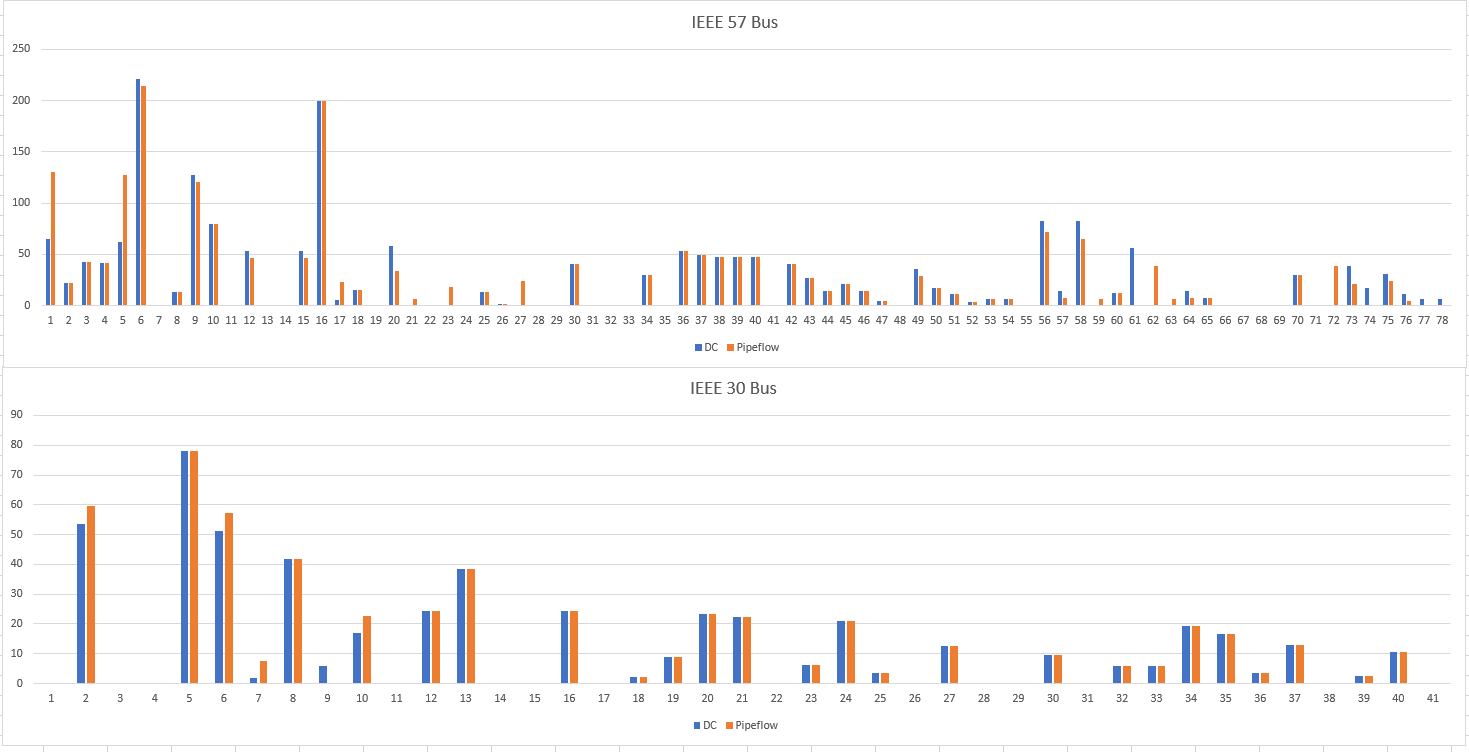
\includegraphics[width=\linewidth]{DCvsPipeflow.PNG}
		\caption{Comparison of DC and traditional (pipeflow) network flow}
	\end{figure}
	
	\subsubsection{DCOPF}
		To begin looking at methods of studying repair of damaged power grids, we first must understand the Direct Current-Optimal Power Flow (DC-OPF) model as it forms the basis of all more complex power models used in this thesis.
		
	We define the following variables and sets
	\begin{itemize}
		\item $C_i$ is the cost of producing one unit of power at node i
		\item $P_i$ is the maximum power generation for node i
		\item $G_i$ is the power generated at node i
		\item $\theta_i$ is the phase angle for power flow at node i 
		\item $D_i$ is the demand for power at node i
		\item $B_e$ is the line susceptance for power line e
		\item $X_e$ is the power flow on line e
		\item $\underline{L_e}$ is the maximum amount of flow on line e
		\item $i \in N$ is the set and indexer for nodes
		\item $e \in E$ is the set and indexer for edges
	\end{itemize}
	We also use the following notation for clarity in models
	\begin{itemize}
		\item $o(e)$ is the node at the origin of line e
		\item $d(e)$ is the node at the destination of line e
		\item $O(i)$ is the set of lines with origin i
		\item $D(i)$ is the set of lines with destination i
	\end{itemize}
	The model can then be formulated as 
	\begin{equation}
Minimize \sum_{i\in N} C_i G_i
	\end{equation} 
	subject to
	\begin{eqnarray}
	X_e = B_e (\theta_{o(e)} - \theta_{d(e)}), \hspace{4pt} \forall e \in E\\
	G_i - \sum_{e \in O(i)} X_e + \sum_{e \in D(i)} X_e = D_i, \hspace{4pt} \hspace{4pt} \forall i \in N\\
	  G_i \leq P_{i} \hspace{4pt} \hspace{4pt} \forall i \in N	\\ 
	  -\underline{L_e} \leq X_e \leq \underline{L_e}
\end{eqnarray}

To explain, the problem is how to generate power at the minimum cost in a way that satisfies all of the demand subject to the physics of how power grids operate. Constraint $1)$ is part of the DC approximation to AC power flow where we assume $sin(x) = x$ for small values of x and reduce power flow to just its real component and the aforementioned linear approximation of phase angle. Constraint $2)$ is a standard flow balance constraint. Constraint $3)$ restricts generation to the maximum for the generator. Constraint $4)$ is a flow capacity constraint on each power line. While overall a simple problem, it serves as the building block for most of the power grid models used for the rest of this thesis.
	
	
	\subsection{Road Repair Problem}
	When dealing with repairs on the power grid, we need a framework for solving problems based on the damage to the road network. We elect to solve this as a routing problem to plot the tour of a repair crew assigned to clearing debris and dig out minor flooding. 
	
	We model this as per the following:
	
\begin{displaymath}
\begin{array}{ll}
T & \mbox{the set of time periods (shifts) over the time horizon, indexed by $t$}\\
N & \mbox{the set of nodes in the graph, representing the intersections of road segments}\\
c_{ij}^t & \mbox{measure of the value of the road segment from node $i$ to node $j$ during period $t$}\\
l_{ij} & \mbox{is the length of the road segment between nodes $i$ and $j$ when everything is working as normal}\\
r_{ij} & \mbox{time to repair the road segment between nodes $i$ and $j$ (hours), including travel time}\\
s^t & \mbox{the length of period $t$ in time units (hours)}\\
o_{ij} & \mbox{initial condition of the road segment between nodes $i$ and $j$}\\
X_{ij}^t & \mbox{binary variable for road segment $ij$ being operational in time $t$}\\
K_{ij}^t & \mbox{binary variable for travel from $i$ to $j$ being in the tour at time $t$}\\
S_{ij}^t & \mbox{length of travel for road segment $ij$ at time $t$}\\
\end{array}
\end{displaymath}	
\begin{equation}
\min \sum_{t \in T}  \sum_{i,j \in N} c_{ij}(1-X_{ij}^t) 
\end{equation}
subject to:
\begin{eqnarray}
\sum_{i,j \in N} S_{ij}^t K_{ij}^t \leq s^t, \hspace{6pt} \forall t\in T \\
S_{ij}^t = \max \{l_{ij}, r_{ij}(1-X_{ij}^t) \}, \hspace{6pt} \forall t\in T, \hspace{5pt} \forall i,j \in N\\
\sum_{j \in N} K_{ij}^t - \sum_{j \in N} K_{ji}^t = 0, \hspace{6pt} \forall t\in T, \hspace{5pt} \forall i \in N\\
X_{ij}^t \le \sum_{t'=0}^{t-1} K_{ij}^{t'} + o_{ij} , \hspace{6pt} \forall t\in T,  \hspace{5pt} \forall i,j \in N\\
\sum_{i,j \in S; i\neq j} X_{ij}^t \leq |S|-1, \hspace{6pt} \forall S \subset N, \hspace{2pt} S \neq \emptyset, \hspace{5pt} \forall t\in T.
\end{eqnarray}

To explain the modeling, the objective is to maximize the length of in-service road. Without loss of generality, this can be substituted with a set of priority weights from another agency that cares about the road grid's operation.

Constraint 7) provides a scheduling constraint limiting the tour's length to the length of the shift. Constraint 8) is a nonlinear but linearizable constraint that sets the length of a road to either its nominal operation time or its repair time depending on whether or not it's marked as working ($X_{ij}$ = 1). Constraint 9) is a standard path connectivity constraint. Constraint 10) restricts each road segment to only be working if it started working or has been repaired, and Constraint 11) is a standard set of subtour elimination constraints.
	\subsection{Power Grid Repair Problem}
	When looking at repair of the power grid, we formulate a discrete time mixed integer program that captures both the planning/scheduling/movement of repair crews as well as the DC power flow model. We pose the model as follows
	\small
	\begin{displaymath}
	\begin{array}{llll}
	N & \mbox{set of nodes, indexed by $i$} & X_{e}^{t} & \mbox{power flow on line $e$ at time $t$}\\
	E & \mbox{set of power lines, indexed by $e$} & G_{k}^t & \mbox{production from generator $k$ at time $t$}\\
	R & \mbox{the set of road segments} & V_i^t & \mbox{indicator for node $i$ functioning at time $t$}\\
	T & \mbox{the planning horizon, indexed by $t$} & W_{e}^t & \mbox{indicator for line $e$ functioning at time $t$} \\
	O(i) & \mbox{set of lines with origin $i$} & S_{e}^t & \mbox{indicator for line $e$ serviced at time $t$}\\
	D(i) & \mbox{set of lines with destination $i$} & F_i^t & \mbox{indicator for node $i$ serviced at time $t$}\\
	o(e) & \mbox{origin node of line $e$} & \theta_i^t & \mbox{phase angle for the power flow at $i$ in time $t$}\\
	d(e) & \mbox{destination node of line $e$} & MST_t & \mbox{length of the tree used for ``routing'' at $t$} \\
	\underline{L_e},\overline{L_e} & \mbox{power lower and upper bounds for line $e$}& Z_{ij}^t & \mbox{indicator for $ij$ being in the spanning tree at $t$}\\
	\Delta_{i} & \mbox{time to repair node $i$} \\
	\delta_{e} & \mbox{time to repair line $e$}\\
	C_{SP(i)} & \mbox{length of the shortest path from depot to node $i$}\\
	D_i & \mbox{power demand at node $i$ in the pre-disaster state}\\
	P_k & \mbox{maximum power generation for generator $k$}\\
	B_e&  \mbox{line susceptance for power line $e$}\\
	I_e, I_i & \mbox{initial condition of line $e$ and node $i$, respectively}
	\end{array}
	\normalsize
	\end{displaymath}
	\begin{equation}
	\min \sum_{i \in N} \sum_{t \in T} (1-V_i^t)D_i
	\end{equation}
	subject to:
	\begin{eqnarray}
	X_e^t = B_e (\theta_{o(e)}^t - \theta_{d(e)}^t), \hspace{5pt} \forall t \in T, \hspace{4pt} \forall e \in E\\
	G_i^t - \sum_{e \in O(i)} X_e^t + \sum_{e \in D(i)} X_e^t = D_iV_i^t, \hspace{4pt} \forall t \in T, \hspace{4pt} \forall i \in N\\
	G_k^t \leq P_{k} V_{k}^t, \hspace{4pt} \forall t \in T, \hspace{4pt} \forall k \in N\\
	\underline{L_e}W_{e}^t \leq X_{e}^t \leq \overline{L_e}W_{e}^t, \hspace{4pt} \forall t \in T, \hspace{4pt} \forall e \in E\\
	\underline{L_e}V_{o(e)}^t \leq X_{e}^t \leq \overline{L_e}V_{o(e)}^t, \hspace{4pt} \forall t \in T, \hspace{4pt} \forall e \in E\\
	\underline{L_e}V_{d(e)}^t \leq X_{e}^t \leq \overline{L_e}V_{d(e)}^t, \hspace{4pt} \forall t \in T, \hspace{4pt} \forall e \in E\\
	MST^t = \sum_{i \in N} \sum_{j \in N} SP_{ij}^t Z_{ij}^{t},  \hspace{4pt} \forall t \in T\\
	\sum_{i \in N} \sum_{j \in N} Z_{ij}^{t} = \sum_{i \in N} F_i^t + \sum_{e \in E} S_e^t - \sum_{i \in N} F_i^t \sum_{e \in O(i)} S_e^t - \sum_{i \in N} F_i^t \sum_{e \in D(i)} S_e^t, \hspace{6pt} \forall t \in T\\
	\sum_{i,j \in S} Z_{ij}^t \leq |S|-1, \hspace{6pt} S \subset N, \hspace{2pt} S \neq \emptyset, \hspace{5pt} \forall t\in T \\
	\sum_{j \in N} Z_{ij}^t \leq F_i^t + \sum_{e \in O(i) \cup D(i)} S_{e}^t, \hspace{6pt} \forall t \in T, \hspace{4pt} \forall i \in N \\
	\sum_{e \in E} \delta_{e}S_e^t + \sum_{i \in N}\Delta_{i}F_i^t + MST_t \le s^t, \hspace{6pt} \forall t \in T\\
	V_i^t \leq \sum_{t'=0}^{t-1} F_i^{t'}+I_i, \hspace{4pt} \forall i \in N\\
	W_{e}^t \leq \sum_{t'=0}^{t-1} S_{e}^{t'}+I_e, \hspace{4pt} \forall e \in E
	\end{eqnarray}
	
	Constraint 13) is the same constraint from the DCOPF model above to handle line susceptance and phase angle related power flow. Constraint 14) is the flow balance constraint from DCOPF with the alteration that demand can be switched on and off at penalty to the objective. Constraint 15) is a generation capacity constraint where generation of power can only flow into the grid if the bus that the generator connects to is intact. Constraints 16-18) are flow limit constraints subject to functioning of the line and buses on both sides of the line.
	
	Constraint 19) defines the length of a minimum spanning tree based on what elements are put in. Constraint 20) is a quadratic constraint that counts how many elements need to be inserted into the minimum spanning tree. Constraint 21) is a standard subtree elimination constraint. Constraint 22) restricts the inclusion of elements in the tree to only nodes that have a repair at them. Constraint 23) is a scheduling constraint that matches the one seen in the road repair model, and constraints 24-25) are functionality constraints that restrict operation to things that either started working or have been repaired.
	\subsection{Lower Bounding and Post Processing Heuristic}
	
	From the above models, we also recognize that we can generate a lower bound using these models. By setting all road lengths to zero, we can then generate a schedule for repairs that would satisfy flow constraints and minimize shed demand. This can be post processed into a feasible schedule by starting with the lower bound schedule and then repacking it into shifts using the following algorithm:
	\begin{enumerate}
		\item Begin by assigning shift 1 as the current working shift
		\item Move any repair that hasn't been done that is on the feasible list onto the priority list
		\item Assign any repair from the lower bound's working shift that would occur in the current working shift to the feasible list.
		\item starting from the depot as the current node, calculate the time to reach and repair every element on the priority list from the current node.
		\item if there are unassigned nodes on the priority list that will fit into the current shift, assign the lowest cost node that will. Update the current node to be that node. Go back to step 4 
		\item if there are unassigned edges on the priority list that will fit into the current, assign the lowest cost edge, update the current node, then go back to step 4.
		\item if there are unassigned nodes on the feasible list that will fit into the current, assign the lowest cost node, update the current node, then go back to step 4.
		\item if there are unassigned edges on the feasible list that will fit into the current, assign the lowest cost edge, update the current node, then go back to step 4.
		\item If nothing else will fit into the current shift, increment to the next shift and start from step 2.
		\item Once every repair has been assigned to a shift, end the algorithm.
	\end{enumerate}
	
	This is very similar to most greedy heuristics for knapsack problems just with a linked series of knapsacks. This heuristic runs in polynomial time (for the heuristic itself, the simplified mixed integer program is non-polynomial though fast), and as we show later, it's close to our full solutions in a variety of examples
	
	\subsection{Framework for interacting}
	Now that we've established both models to be used to draw insights from this problem, we now outline how we're going to interact them. Since the models are solved independently, we have to choose one of them to be the first mover and one to be the second mover. We therefore lay out the following frameworks:
	\begin{itemize}
		\item \textbf{Road First}-- To model the problem as if the road grid's actor had priority in the repair effort. This is done by solving the road model, then feeding the solutions into the power model as a time-varying shortest path.
		\item \textbf{Power First} -- To model the problem with the power grid as the first mover, we solve the power grid repair problem with the roads at their nominal length and presume that due to coordination effects the power grid actor the road grid repairs will happen before the road is needed to affect power repairs. To account for this delay while waiting for road repair, we introduce a one shift delay before the start of power repairs.
		\item \textbf{Uncoordinated Repairs} -- To handle the case where the power agency may have to commence repairs with no prior information about the state of the roads. We model the roads as if they are damaged and their state does not change.
		\item \textbf{Heuristic} -- Using the heuristic described above, both road first and power first versions of the problem can be solved to approximation quickly.
	\end{itemize}
	\section{Results on Standard test systems}
	\subsection{Introduction to Results}
	To validate the model outlined as more than just a theoretical exercise in modeling, we engineer test cases based on standard IEEE power grids. We choose to use the 30 bus and 57 bus systems \$CITATION GOES HERE in order to capture things on a large enough scale to demonstrate applications for extension into practical uses later on. To convert these from standard test grids to DC versions for use in this model, reactive/imaginary power flow is dropped leaving only real power flow. We then overlay a Watts-Strogatz graph as mentioned earlier based on fitting power buses to a grid. The key reason for this is to maintain triangle inequalities where having a network that violates triangle inequalities is both unrealistic to "real world" situation as well as altering the solutions of routing problems \cite{FlemingEA2013}. We plan this so that travel time between opposite sides of the network are about 3 hours so that routing times are not trivial compared to repair times.
	
	To show validity, we first solve out a base damage scenario for both grid topologies, then conduct perturbations of respectively weather damage, road topology, and damage intensity to show that the model is valid for a large variety of inputs. 
	
	Looking at our first case to validate the model, we apply geographically clustered damage to both road. 
	
	

	\section{Resilience}
	\subsection{Introduction}
	Given that we've constructed a model for response to a scenario of a hurricane strike on a grid, we can use this to look at how different methods of resilience. By generating test cases and then making the grid resilient through either traditional hardening or by forming microgrids as has become popular in electrical engineering literature.
	\subsection{Hardening}
	
	Hardening is one of the approaches to resilience by fortifying a subset of nodes and edges in a network to make it harder to damage. Traditionally this is looked at in the context of interdiction problems \cite{ChurchEA2007}. To overview the problem solved in hardening: player 1 operates a network, player 2 attacks the network with the objective of minimizing maximum flow, player 1 hardens the network before the attack under the assumption that it's coming. This serves as a max/min/max tri-layer optimization problem.
	
	A similar approach can be taken with disaster planning. Unlike in multi-actor interdiction, the attack coming from a hurricane is a random process of nature and not a targeted interdiction by an intelligent actor. When solving this problem, finding a fixed quantity of damage equal to the ability to fortify under budget constraints that minimizes maximum flow allows for planning of network hardening. Solving this to optimality requires a delve into bi-level optimization that is outside the scope of this thesis. We therefor solve the problem heuristically through the following setup.
	
	\begin{enumerate}
		
	\item Solve baseline DC-OPF for the grid
	\item identify how many nodes (n) and edges (e) to be fortified
	\item select the 2n highest demand nodes and the 2e highest utilization edges
	\item for each subset of nodes/edges of the correct size, solve DC-OPF with those elements damaged
	\item find the minimum demand satisfied and use those damaged elements as the fortified elements when analyzing resilience 
	\end{enumerate}
		
	\subsection{Microgriding/Islanding}
	\section{Conclusions}
	\subsection{Results}
	\subsection{Future Research Direction}
	\section{Bibliography}
	\bibliographystyle{siam}
	\bibliography{sources}
\end{document}